\documentclass[runningheads]{llncs}
\usepackage{graphicx}
\usepackage{amsmath,amssymb}
\usepackage{booktabs}
\usepackage{url}
\begin{document}
\title{Optimising a Flappy Bird Controller with Random Search, Differential Evolution and Particle Swarm Optimisation}
\titlerunning{Optimising a Flappy Bird Controller}
\author{[Group members to add]}
\authorrunning{[Group members to add]}
\institute{[Group number to add]}
\maketitle
\begin{abstract}
This report investigates how Random Search (RS), Differential Evolution (DE) and particle swarm optimisation (PSO) can be used to find a controller for Flappy Bird. The experiments examine how the choice of observations, game difficulty and optimiser settings affect performance. Controller weights are found with a fixed number of game episodes, and the resulting controllers are tested on fresh episodes. [Add results and conclusion after all experiments are complete.]
\end{abstract}

\section{Introduction}
The aim is to find weights for a simple Flappy Bird controller. At each step, the controller receives information about the game and chooses whether to flap or do nothing. RS, DE and PSO search for weights that earn a high game reward. The experiments also examine how performance changes with the observations, the width of the pipe gaps and the optimiser settings. The game runs in Gymnasium \cite{towers2024gymnasiumstandardinterfacereinforcement}.

\section{Problem Description}
The controller receives either 12 descriptive features, including the bird's position and speed, or lidar distances to obstacles. The lidar observations contain 4, 8 or 12 evenly spaced readings. The controller scores the two actions, flap and do nothing, and chooses the higher scoring one. For an observation $s\in\mathbb{R}^{m}$ and weights $W\in\mathbb{R}^{m\times 2}$, the selected action is $a=\arg\max_{j\in\{0,1\}}(W^\top s)_j$. This gives 8, 16 and 24 weights for the lidar settings and 24 weights for the feature setting.

The game awards $+0.1$ for each frame survived and $+1$ for passing a pipe. It gives $-1$ for dying and $-0.5$ for touching the top of the screen. The total episode reward is the fitness score. Pipe positions vary between games, while \texttt{pipe\_gap} sets the width of the opening. Changing the number of lidar readings changes both the number of weights and the information available to the controller.

\section{Experiments}
PSO searches for controller weights that give a high episode reward. It tracks each particle's best position and the best position found by the swarm. Particle positions and velocities are updated as follows:
\begin{align}
v_{id}^{t+1}&=w v_{id}^{t}+c_1r_{1,id}(p_{id}-x_{id}^{t})+c_2r_{2,id}(g_d-x_{id}^{t}),\\
x_{id}^{t+1}&=x_{id}^{t}+v_{id}^{t+1}.
\end{align}
Here $p$ is a particle's best position, $g$ is the swarm's best position, and each $r$ is a new uniform random value. Initial positions were between $-1$ and $1$, and initial velocities were between $-0.2$ and $0.2$. Positions and velocities were clipped to these ranges after each update. Unless varied, PSO used six particles, $w=0.7298$ and $c_1=c_2=1.49618$. Each run used 30 game episodes, including the initial evaluation of every particle. Each setting was repeated with PSO seeds 101, 202 and 303. The returned controller was then tested on two fresh episodes. The tables give the mean test reward for each run, followed by the mean and sample standard deviation across runs. ``Search best'' is the highest reward observed during optimisation.

\begin{table}[t]
\caption{PSO experimental settings. Every row uses 30 search episodes per trial, three trials and two fresh test episodes per returned controller. Unlisted PSO parameters use the defaults above.}
\centering\small
\begin{tabular}{lll}
\toprule
Study & Observation and game & Varied PSO setting \\
\midrule
Observation & lidar 4, 8, 12; gap 100 & default \\
Observation & 12 features; gap 100 & default \\
Difficulty & 8 lidar; gaps 80, 100, 120 & default \\
Sensitivity & 8 lidar; gap 100 & swarm 4, 6, 8 \\
Sensitivity & 8 lidar; gap 100 & $w=0.5$ or $c_2=2.0$ \\
\bottomrule
\end{tabular}
\end{table}
The gap 100 setting appears in more than one experiment batch. These are separate runs with different game episodes. A PSO seed controls the optimiser's random choices, but game episodes are reset without a seed. Two runs with the same PSO seed can therefore receive different rewards. Episode length also varies because controllers survive for different numbers of frames.

\paragraph{Random Search and Differential Evolution.}

\section{Results}
\begin{figure}[t]
\centering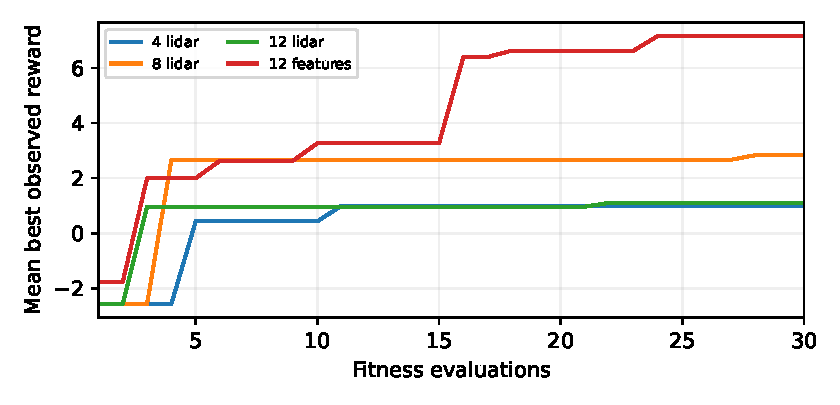
\includegraphics[width=.82\textwidth]{figures/convergence.pdf}
\caption{Mean best observed search reward against episode evaluations for observation settings at pipe gap 100. Six particles, default coefficients, 30 evaluations and three trials per curve. Curves describe selected noisy episode returns, not fresh controller performance.}
\end{figure}
The lines in the figure only rise because PSO remembers its highest score so far. One high scoring episode has a noticeable effect on the 8 lidar line. Fresh episodes provide a separate check of the returned controller, although two episodes give only a rough estimate of its usual performance.

\begin{table}[t]
\caption{Observation study at pipe gap 100. Default PSO, 30 search evaluations per run, three runs and two fresh episodes per returned controller. Entries are mean $\pm$ sample standard deviation across run means; rewards are episode totals.}
\centering\small
\begin{tabular}{lrrr}
\toprule
Observation & Weights & Search best & Fresh reward \\
\midrule
4 lidar & 8 & $1.00\pm0.35$ & $1.03\pm0.40$ \\
8 lidar & 16 & $2.83\pm3.52$ & $1.77\pm1.67$ \\
12 lidar & 24 & $1.10\pm0.52$ & $0.73\pm0.12$ \\
12 features & 24 & $7.17\pm5.71$ & $4.80\pm3.34$ \\
\bottomrule
\end{tabular}
\end{table}
The controller using descriptive features had the highest average fresh reward. It uses the same number of weights as the 12 lidar controller, which suggests that the type of information matters. Three runs are too few to establish whether features generally perform better. The lidar results do not steadily improve or worsen as readings are added. Variation at 8 readings is especially large, so these results do not show a clear effect of dimension.

\begin{table}[t]
\caption{Difficulty study with 8 lidar readings (16 weights). Default PSO, 30 evaluations, three runs and two fresh episodes per returned controller. Values are mean $\pm$ sample standard deviation across run means.}
\centering\small
\begin{tabular}{rrr}
\toprule
Pipe gap & Search best & Fresh reward \\
\midrule
80 & $0.97\pm0.29$ & $0.55\pm0.43$ \\
100 & $2.23\pm2.48$ & $2.78\pm3.44$ \\
120 & $35.70\pm60.45$ & $3.68\pm4.99$ \\
\bottomrule
\end{tabular}
\end{table}
Average fresh reward increased with the pipe opening width. At gap 120, the best search reward was much higher than the fresh test reward and varied greatly between runs. One unusually favourable episode may have contributed to this difference. The two gap 100 batches also gave different averages under the same settings, showing how much these small samples can vary with the pipe sequences.

\begin{table}[t]
\caption{PSO sensitivity with 8 lidar readings, gap 100, 30 evaluations, three runs and two fresh episodes per controller. Fresh reward is mean $\pm$ sample standard deviation across run means. Other coefficients retain their defaults.}
\centering\small
\begin{tabular}{lr}
\toprule
Setting & Fresh reward \\
\midrule
Swarm 4 & $1.48\pm1.18$ \\
Swarm 6, baseline & $1.27\pm0.81$ \\
Swarm 8 & $1.52\pm1.24$ \\
Swarm 6, $w=0.5$ & $1.02\pm0.38$ \\
Swarm 6, $c_2=2.0$ & $2.82\pm2.83$ \\
\bottomrule
\end{tabular}
\end{table}
Changing the PSO settings did not give a clear winner. The higher social coefficient had the best average in these runs, but its results also varied the most. Each setting was tested only three times. With the same episode budget, a larger swarm also allows fewer update rounds.

\paragraph{Comparison with RS and DE.}

\section{Impact of Dimensionality}
Wang et al. \cite{wang2016rembo} study optimisation in a space with many variables when only a few combinations of those variables affect the result. They call the size of this smaller space the effective dimension. Their method, REMBO, searches a randomly chosen lower dimensional space instead of searching every variable directly. They tested it on artificial functions and on the settings of a mixed integer solver. Performance was measured by the quality of the solution found after a given number of function evaluations. Their results show that a large search space can still be manageable when its effective dimension is low.

The distinction between the number of variables and the effective dimension is useful here, but it is unknown whether this Flappy Bird controller has a low effective dimension. Several embedding sizes would need to be tested before using REMBO for this problem. Controllers would also need evaluation on fresh games, since noisy rewards could make a method appear better than it is. In these experiments, changing the lidar count changes both the number of weights and the information available to the controller. The feature and lidar controllers with the same number of weights performed differently, so the lidar comparison is not a pure test of dimension.

\section{Conclusion}

\bibliographystyle{splncs04}
\bibliography{bibliography}
\end{document}
